\documentclass[11pt,a4paper]{article}

\usepackage[utf8]{inputenc}
\usepackage{graphicx}
\usepackage[spanish]{babel}
\usepackage{float}				%Para poner las imagenes exactamente donde se me cante las pelotas en caso de quererlo, poniendole [H]
\usepackage{amsmath}
\usepackage{epstopdf}
\usepackage{geometry}
\usepackage{hieroglf}
\usepackage{subcaption}
\usepackage[justification=centering]{caption}
\usepackage[colorinlistoftodos]{todonotes}
\usepackage[colorlinks=true, allcolors=blue]{hyperref}
\geometry{
a4paper,
left=20mm,
right=20mm,
top=25mm,
bottom = 20mm
}
\usepackage{float}
\usepackage{units}
% \usepackage{hyperref}   %Esto es para ir a los links

\newcommand{\rojo}[1]{\textcolor{red}{#1}}    % Comando para escribir texto en rojo




\title{\textbf{Matemática de los Sistemas Biológicos \\ Práctica 1 - Modelos de una sola población}}

\author{
{F. M. Cabrera}
%[1ex] \small{\textit{ Facultad de Ciencias Exactas y Naturales.}} \\
%\small{\textit{Universidad de Buenos Aires. Ciudad Universitaria. Pabellón I. Buenos Aires. Argentina}}
}
\date{\textit{\today}}


% Esto modifica el interlineado
\renewcommand{\baselinestretch}{1}

\graphicspath{{Figuras/}}

\begin{document}

\maketitle

%\thispagestyle{empty} 


\setcounter{page}{1}

%\begin{abstract}


%\end{abstract}
%\vspace*{1cm}

Todo el código implementado en esta practica puede encontrarse \href{https://github.com/cabre94/MSB_IB}{acá}.


\section*{Ejercicio 1}
\graphicspath{{Figuras/ej_01/}}

Hola \cite{einstein}

El mapeo de Beverton-Holt es
\begin{equation}
    n_{t+1} = f(n_{t}) = \frac{rn_{t}}{1+\frac{r-1}{K}n_{t}}.
\end{equation}

En donde para encontrar los puntos buscamos los $n^{*}$ tal que $f(n^{*}) = n^{*}$, obteniendo que $n^{*} = 0$ y $n^{*} = K$ son los puntos fijos del sistema. Para estudiar la estabilidad, calculamos la derivada de $f(n_{t})$
\begin{equation}
    f^{'}(n_{t}) = \frac{r}{(1+\frac{r-1}{K}n)^{2}}
    \label{eq:Mapeo_Beverton-Holt}
\end{equation}
la cual evaluada en los puntos fijos obtenemos que $f'(n_{t}=0) = r$, con lo cual $n^{*}=0$ es estable si $|r|<1$ e inestable si $|r|>1$. Por otra parte, para $n^{*}=K$ obtenemos que $f'(n_{t}=K)=\dfrac{1}{r}$ con lo cual es inestable si $|r|<1$ y estable si $|r|>1$.

Pasemos a ver la el comportamiento del mapeo obtenido numéricamente. En la Figura \ref{01_Simulacion} se observa la evolución del sistema para distintas condiciones iniciales (todas positivas, ya que $n$ representa poblaciones) para $r=2$ y $K=1$, mientras que en la Figura \ref{01_Coweb} se observa un gráfico \textit{Coweb} para los mismos parámetros. De estos resultados se observa que $n^{*}=0$ es un equilibrio estable (acorde al hecho de que $|r|>1$) y $n^{*}=K=1$ es un equilibrio estable.

\begin{figure}[hbt!]
    \centering
    \begin{subfigure}[b]{0.49\textwidth}
        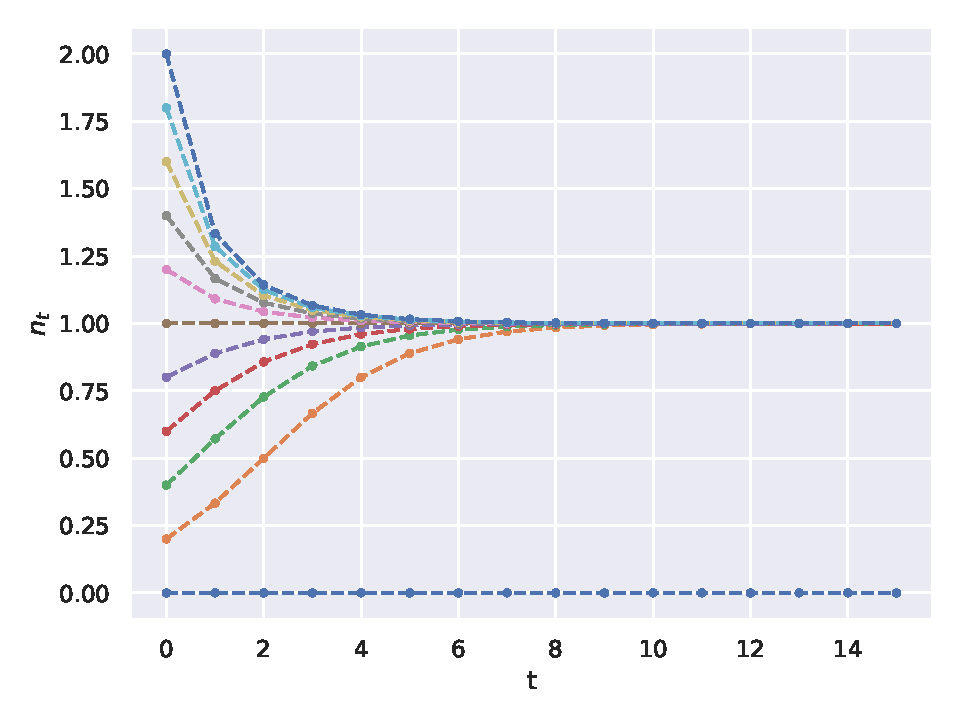
\includegraphics[width=\textwidth, height=0.8\textwidth]{Mapeo_r=2.pdf}
        \caption{}
        \label{01_Simulacion}
    \end{subfigure}
    \hfill
    \begin{subfigure}[b]{0.49\textwidth}
        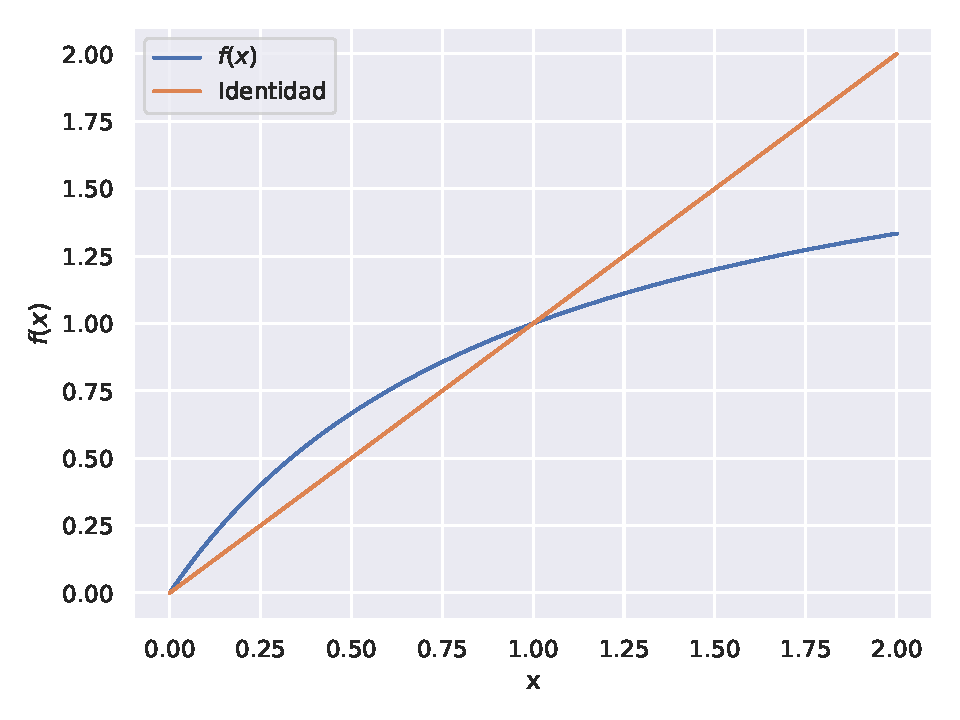
\includegraphics[width=\textwidth, height=0.8\textwidth]{Coweb_r=2.pdf}
        \caption{}
        \label{01_Coweb}
    \end{subfigure}
    \caption{Ene  la Figura (a) se observa la evolución del sistema para distintas condiciones iniciales para $r=2$ y $K=1$, mientras que en la Figura (b) se observa un gráfico \textit{Coweb} para los mismos parámetros.}
    \label{PONER_LABEL}
\end{figure}

\rojo{Falta mostrar que pasa para $r<1$. Acalrr lo del signo de K.}

En caso de que $r=1$, la Ec. \ref{eq:Mapeo_Beverton-Holt} se reduce a $n_{t+1} = n_t$, en donde todos los $n$ son puntos fijos, pero el comportamiento no es muy interesante.
\section*{Ejercicio 2}
\graphicspath{{Figuras/ej_02/}}

Tenemos la ecuación logística con retraso
\begin{equation}
    \frac{dN}{dt} = r N(t) \left[1- \frac{N(t-T)}{K}\right]
\end{equation}
la cual se resolvió numéricamente usando diversos valores de los parámetros. En la Figura \ref{02_ejercicio} se observa las simulaciones obtenidas para tres valores del parámetro $r$: $0.3$, $1.2$ y $2$. En todos los casos $T=1$, $K=10$ y $N(t)=2$ para $-T < t \leq 0$. Para $r$ chicos ($r=0.3$), se observa que el sistema presenta un régimen monótono en donde la población tiende al valor de $K$, como la ecuación logística. Luego, al aumentar $r$, primero se observan oscilaciones amortiguada y al seguir aumentando $r$ pasan a observarse oscilaciones sostenidas. Según \cite{Chule},  para $0<rT<e^{-1}$ el sistema posee un comportamiento monótono. Para $e^{-1} < rT < \dfrac{\pi}{2}$ el sistema presenta oscilaciones amortiguadas y por ultimo para $\dfrac{\pi}{2} < rT$ se obtienen oscilaciones sostenidas.

\begin{figure}[h!]
    \centering
    \includegraphics[width=0.5\textwidth]{Regimenes.pdf}
    \caption{Resolución numérica para la ecuación logística con retraso variando el parámetro $r$. Se observan los regímenes monótono, oscilatorio amortiguado y oscilatorio sostenido para $r$ igual a $0.3$, $1.2$ y $2$, respectivamente. $T=1$, $K=10$ y $N(t)=2$ para $-T < t \leq 0$.}
    \label{02_ejercicio}
\end{figure}

Tenemos una aproximación analítica para cuando $T$ es un poco mayor que que el valor critico $T_c = \nicefrac{\pi}{2r}$, la cual viene dada por
\begin{equation}
    N(t) \approx K + C e^{ \frac{\epsilon t}{1 + \nicefrac{\pi^{2}}{4}} } e^{it \left[ 1- \frac{\epsilon \pi}{2 ( 1 + \nicefrac{\pi^{2}}{4})} \right]}
    \label{02_Ec_Aproximada}
\end{equation}
en donde $T = T_c + \epsilon$ (es decir que la aproximación es valida para el régimen de oscilaciones sostenidas). En la Figura \ref{02_Comp_Analitica} se observa una comparación entre la simulación numérica y la solución aproximada valida para $r=2$ y $\epsilon=0.01$. Se observa que la solución analítica aproximada no logra reproducir correctamente la amplitud de las oscilaciones, pero si es posible estimar el periodo de las mismas. En particular, debido al termino $e^{ \frac{\epsilon t}{1 + \nicefrac{\pi^{2}}{4}} }$ de la Ec. \ref{02_Ec_Aproximada}, la solución aproximada diverge para $t\rightarrow \infty$.

\begin{figure}[h!]
    \centering
    \begin{subfigure}[b]{0.48\textwidth}
        \includegraphics[width=\textwidth]{Comp_Analitica_2.pdf}
        \caption{}
        \label{02_Comp_Analitica}
    \end{subfigure}
    \hfill
    \begin{subfigure}[b]{0.48\textwidth}
        \includegraphics[width=\textwidth]{Amplitud_r=2.0.pdf}
        \caption{}
        \label{02_Picos}
    \end{subfigure}
    \caption{En (a) se observa una comparación entre la simulación numérica y la solución aproximada valida para el régimen de oscilaciones sostenidas para $r=2$ y $\epsilon=0.01$. Se observa que la solución analítica aproximada no logra reproducir correctamente la amplitud de las oscilaciones, pero si es posible estimar el periodo de las mismas. En (b), se observa una simulación y la obtención de los picos y valles de las oscilaciones para el calculo de la amplitud de las oscilaciones y su periodo.}
    \label{02_ejercicio_2}
\end{figure}

Luego se procedió a verificar que la amplitud de las oscilaciones es independiente de las condiciones iniciales y que el periodo de las oscilaciones es independiente de $r$. Para ambos casos, se realizo una simulación variando la condición inicial o $r$ según corresponda y se obtuvieron los picos y valles de las oscilaciones para determinar la amplitud y periodo. Un ejemplo del resultado obtenido puede observarse en la Figura \ref{02_Picos}.

\begin{figure}[h!]
    \centering
    \begin{subfigure}[b]{0.48\textwidth}
        \includegraphics[width=\textwidth]{Amplitud_Barrido.pdf}
        \caption{}
        \label{02_Barrido_CI}
    \end{subfigure}
    \hfill
    \begin{subfigure}[b]{0.48\textwidth}
        \includegraphics[width=\textwidth]{Periodo_Barrido.pdf}
        \caption{}
        \label{02_Barrido_r}
    \end{subfigure}
    \caption{En (a) se observa el valor obtenido de las distintas amplitudes en función de las distintas condiciones iniciales. Se observa que la amplitud presenta pequeñas variaciones del orden de $7\times 10^{-4}$. Por otro lado, como puede observarse en (b), el periodo de las oscilaciones no son invariantes respecto al valor de $r$.}
    \label{02_Resutados_Barridos}
\end{figure}

En la Figura \ref{02_Barrido_CI} se observa el valor obtenido de las distintas amplitudes en función de las distintas condiciones iniciales. Se observa que la amplitud presenta pequeñas variaciones del orden de $7\times 10^{-4}$. Por otro lado, como puede observarse en la Figura \ref{02_Barrido_r}, el periodo de las oscilaciones no son invariantes respecto al valor de $r$.
\section*{Ejercicio 3}
\graphicspath{{Figuras/ej_03/}}


\section*{Ejercicio 4}
\graphicspath{{Figuras/ej_04/}}

Tenemos una especie con un ciclo de vida anual en la que cada individuo produce $r$ descendientes y luego muere, cuya evolución describimos como
\begin{equation}
    N_{t+1} = r N_{t}
    \label{04_Modelo}
\end{equation}
y en donde $r$ obedece a una distribución de Poisson con media $1.7$.

Simulando el sistema con 1 solo individuo como condición inicial, se observan tres comportamientos distintos según $r$ sea $0$, $1$ o mayor que $1$. Estos tres comportamientos pueden observarse en la Figura \ref{04_Simulacion}. Para $r>1$, la población crece en cada ciclo, mientras que si $r=1$ la población se mantiene, observándose escalones en la evolución de la especie, como se observa para $t$ entre 3 y 6 en la figura. Por ultimo, para el primer ciclo en donde $r=0$, la población se extingue y sin importar el valor de $r$ para iteraciones posteriores, se mantiene en $0$. 

\begin{figure}[h!]
    \centering
    \includegraphics[width=0.6\textwidth]{Simulacion1.pdf}
    \caption{Evolución del sistema para el modelo \ref{04_Modelo} en donde $r$ obedece a una distribución de Poisson con media $1.7$. Se observan tres comportamiento cualitativamente distintos. Para $r>1$, la población crece, para $r=1$ la población se mantiene y se observan escalones en la evolución del sistema y por ultimo para $r=0$ la especie se extingue.}
    \label{04_Simulacion}
\end{figure}

En general, estudiando la evolución del sistema a lo largo de 20 ciclos, se observa que la especie no logra sobrevivir. Veamos porque sucede esto. La densidad de probabilidad es $\frac{e^{-\lambda}\lambda^{k}}{k!}$, con lo cual la probabilidad de que en un ciclo $r$ sea $0$ es $e^{-1.7}\approx0.183$. Entonces, la probabilidad de que $r$ sea distinto de cero en 20 ciclos es $(1-e^{-1.7})^{20}\approx0.01769$. Es decir que la probabilidad de que la especie sobreviva luego de 20 ciclos es de $1.769\%$. Generando cien millones de simulaciones, se obtuvo que en un $1.767\%$ la especie logra sobrevivir, corroborando el calculo previamente descripto. 
\section*{Ejercicio 5}
\graphicspath{{Figuras/ej_05/}}

La ecuacnion logistica presenta dos puntos fijos, en $0$ y $K$.
%  Si $r<0$, estos puntos son estables e inestables respectivamente, con lo cual la evolucion del sistema entre catastrofes es decreciente 
Empecemos por el caso en donde $r > 0$, de manera que $0$ es un punto inestable y $K$ un punto estable. En esta situacion, el rango de valores que nos va a interesar estudiar sera entre 0 y $K$, que es donde la evolucion de la poblacion (entre catastrofes) crece, y queremos estudiar si este crecimiento es suficiente como para sobrellevar las sucesivas redduciones de la pobalcion debido a las catastrofes . Para $N > K$, la poblacion decrece tendiendo a $K$, con lo cual esperamos que tarde o temprano la pobalcion caiga en el rango entre $0$ y $K$.

\begin{equation}
    N(t) = \frac{N_{0} K e^{rt}}{K+N_{0}(e^{rt}-1)}
    \label{eq:Logistica_Sol_Exacta}
\end{equation}

Veamos si podemos obtener una condicion para la cual la especie que estamos modelando puede sobrevivir. Tenemos que los desastres ocurren con una frecuencia promedio $\lambda$, con lo cual el tiempo promedio entre desastres es $\dfrac{1}{\lambda}$. Entonces, utilizando la solución exacta del modelo logistico dada por la Ec. \ref{eq:Logistica_Sol_Exacta}, podemos obtener cuanto logra recuperarse la especie entre catastrofes, en promedio, tomando $t=\dfrac{1}{\lambda}$. Entonces
\begin{equation}
    N(t=\frac{1}{\lambda}) = \frac{pN_{0} K e^{\frac{r}{\lambda}}}{K+N_{0}(e^{\frac{r}{\lambda}}-1)} = \frac{pN_{0} e^{\frac{r}{\lambda}}}{1+N_{0}\frac{e^{\frac{r}{\lambda}}-1}{K}} 
\end{equation}
en donde $N_{0}$ es el valor de la poblacion inmediatamente despues de la ultima catastrofe y en donde ya aplicamos el factor $p$ correspondiente a la la siguiente catastrofe. Esta ecuacion nos dice, en promedio, cuanto aumenta la poblacion entre dos catastrofes. En particular, para analizar si la especie sobrevive o no, nos puede resultar mas util estudiar la situacion critica en donde $N_{0}$ es muy chico, ya que si la especie se extingue es esperable encontrarse en esta situacion tarde o temprano. En este caso, podemos aproximar el denominador por 1 ya que $\frac{1}{1+ax} \approx 1 + ax + \mathcal{O}(x^2)$, con lo cual nos queda que el cambio en la poblacion de la especie entre cada catastrofe es, en promedio,
\begin{equation}
    N(t) = pe^{\dfrac{r}{\lambda}N_{0}}.
\end{equation}
De manera que, cuando la especie esta cerca de extinguirse, la población luego de una catastrofe en proporcional a la pobalcion luego de la catastrofe anterior, en un factor $pe^{\dfrac{r}{\lambda}}$. Entonces, lo que determina que la especie sobreviva o no, sera este factor. Si es menor que 1, cuando la pobalcion esta cerca de la extincion, el sistema siempre seguira decreciendo, con lo cual la extencion es inevitable. En cambio, si este factor es mayor que 1, la poblacion crecera cuando este cerca de la extinción. De manera que la condicion para recuperarse de un desastre sera
\begin{equation}
    pe^{\frac{r}{\lambda}} > 1.
\end{equation}

Para ver esto numericamente, vamos a tomar $r=1$ y $p=\dfrac{1}{e}\approx0.37$, es decir que la poblacion luego de una catastrofe se reduce a casi poco mas de un tercio. Con estos parametros, la condicion para que la especie sobreviva se reduce a $\lambda<1$. En la Figura \ref{05_ejercicio}, se observan las simulaciones obtenidas para tres valores de $\lambda$. Para $\lambda=0.9$, se observa que la poblacion, si bien en ciertos momentos presentan una reduccion, logra reestablecerse sin problema. Para $\lambda=0.95$ comienzan a observarse ciertos intervalos, como por ejemplo el intervalo $100<t<150$, en donde la poblacion esta cerca de extinguirse pero logra recuperarse ya que en el entorno a $N=0$ donde el comportamiento de la poblacion es lineal, esta crece. Por ultimo, para $\lambda=1.05$, en donde ya no se cumple la condicion para la supervivencia de la especie, se observa que una vez que la poblacion se encuentra por extinguirse, no logra recuperarse. 

\begin{figure}
    \centering
    \begin{subfigure}[b]{0.32\textwidth}
        \includegraphics[width=\textwidth]{l=0_9.pdf}
        \caption{$\lambda=0.9$.}
        \label{05_l_9}
    \end{subfigure}
    \hfill
    \begin{subfigure}[b]{0.32\textwidth}
        \includegraphics[width=\textwidth]{l=0_95.pdf}
        \caption{$\lambda=0.95$.}
        \label{05_l_95}
    \end{subfigure}
    \hfill
    \begin{subfigure}[b]{0.32\textwidth}
        \includegraphics[width=\textwidth]{l=1_05_1.pdf}
        \caption{$\lambda=1.05$.}
        \label{05_l_105}
    \end{subfigure}
    \caption{Se observa la simulacion del sistema para tres valores de $\lambda$. Para $\lambda=0.9$ se observa un comportamiento stocastico en donde si bien la poblacion presenta reducciones importantes, en ningun momento esta cerca de extinguirse. Para $\lambda=0.95$, se observa el intervalo $100<t<150$ en donde la poblacion es cercana a cero, pero logra recuperarse. Por ultimo, para $\lambda=1.05$, en donde el factor de la aproximacion lineal pasa a ser menor que 1, se observa que una vez que la poblacion esta cerca de extinguirse, no logra recuperarse.}
    \label{05_ejercicio}
\end{figure}

% \rojo{Podria poner un poco men¿jor los indices como para diferenciar entre catastrofes y demas cosas.}
% \rojo{Poner una nota al pie con la aclaracion del p}
% \rojo{Poner resultados numericos}
\section*{Ejercicio 6}
\graphicspath{{Figuras/ej_06/}}

Tenemos el modelo para describir el efecto Allee
\begin{equation}
    \frac{dN}{dt} = f(N) = r N \left[ 1 - \frac{N}{K} \right] \left[ \frac{N}{A} -1 \right]
\end{equation}
de donde planteando que $f(N) = 0$ obtenemos que los puntos fijos son 0, $A$ y $K$. Para estudiar la estabilidad calculamos la derivada $f'(N)$ obteniendo
\begin{equation}
    f'(N) = r \left[ 1-\frac{N}{K} \right] \left[ \frac{N}{A} -1 \right] + \frac{rN}{A} \left[ 1 - \frac{N}{K} \right] - \frac{rN}{K} \left[ \frac{N}{A}-1\right]
\end{equation}
que evaluando en los puntos fijos obtenidos, tenemos que
\begin{equation}
    f'(N=0) = -r; \indent f'(N=A)=r\left[1-\frac{A}{K}\right]; \indent f'(N=K)=r\left[1-\frac{K}{A}\right]. 
\end{equation}

Para seguir avanzando con el análisis, tomamos el caso en que $r>0$ y $0<A<K$. En esta situación, los puntos fijos en $0$ y $K$ son puntos fijos estables, mientras que el punto fijo en $A$ es inestable. En la Figura \ref{06_Simulacion} se observa la simulación obtenido del sistema para distintas condiciones iniciales. En esta figura se observan dos regímenes, uno en el intervalo $[0,A)$ en donde el sistema evoluciona al equilibrio estable en $0$ y la población se extingue y otro en $[A,\infty)$ en donde el sistema evoluciona al equilibrio estable en $K$ y la población sobrevive. En la Figura \ref{06_Funcion_y_raices} se observa la función que determina la evolución del sistema indicando con flechas sobre el eje de abscisa la evolución del sistema.

\begin{figure}
    \centering
    \begin{subfigure}[b]{0.49\textwidth}
        \includegraphics[width=\textwidth]{Simulacion.pdf}
        \caption{}
        \label{06_Simulacion}
    \end{subfigure}
    % \hfill
    \begin{subfigure}[b]{0.49\textwidth}
        \includegraphics[width=\textwidth]{f.pdf}
        \caption{}
        \label{06_Funcion_y_raices}
    \end{subfigure}
    \caption{En la Figura (a) se observa la evolución del sistema para distintas condiciones iniciales, tomando $r>0$ y $0<A<K$. Se observan dos regímenes, uno en el intervalo $[0,A)$ en donde el sistema evoluciona al equilibrio estable en $0$ y la población se extingue y otro en $[A,\infty)$ en donde el sistema evoluciona al equilibrio estable en $K$ y la población sobrevive. En la Figura (b) se observa la función que determina la evolución del sistema indicando con flechas sobre el eje de abscisa la evolución del sistema. }
    \label{06_ejercicio}
\end{figure}

La diferencia que puede observarse respecto a la ecuación logística, ademas de la aparición de un nuevo punto fijo en $A$, es que la aparición de este nuevo punto fijo genera un cambio en la estabilidad del punto fijo en $0$, el cual es inestable en la ecuación logística mientras que en este caso dicho punto es estable (para $r>0$). De esta forma, como ya se remarco previamente, existe un numero mínimo ($A$) para la población para que la supervivencia sea posible.

En caso de que $0<K<A$, las estabilidades de los puntos fijos en $A$ y $K$ cambian, pero tambien cambian sus posiciones, con lo cual la situacion es analoga a cuando $0<A<K$.
%Por otro lado, si $r<0$, la estabilidad de todos los puntos fijos se invierte


\bibliographystyle{acm}
\bibliography{biblio}

\end{document}



